In this chapter, we will study functions of the form
$$
r(t) = \left(f(t),g(t),h(t)\right) = f(t)\vv i + g(t) \vv j + h(t) \vv k
$$
Such function takes in a parameter $t$ and output a vector.

\section{Limit and Continuity}

\begin{definition}[Limit of vector functions]
If $r(t) = (f(t),g(t),h(t))$, then
$$
\lim_{t\to a} r(t) = \left(\lim_{t\to a} f(t),\, \lim_{t\to a} g(t),\, \lim_{t\to a} h(t)\right)
$$
If $\lim_{t\to a} r(t) = r(a)$, then $r$ is continuous at $a$.
\end{definition}

\subsection{Space Curves}
The graph of a vector function is called the space curve. More formally, for the vector function $r(t)=(f(t),g(t),h(t))$, the set $C$ of all points $(x,y,z)$ such that $x=f(t),\; y=g(t),\;z=h(t)$ for $t$ in the domain of the vector function is the space curve.
$$
C = \{ (x,y,z) \in \R^3 \mid x=f(t),\; y=g(t),\;z=h(t) \text{ for some $t \in D$} \}
$$

\begin{example}[Space curves]
\begin{enumerate}
    \item Circle of radius $r$:
    $$
    x=r\cos t, \qquad y=r\sin t, \qquad z=k
    $$
    for $0 \leq t \leq 2\pi$ and some scalar $k \in \R$.
    
    \item Helix
    $$
    x=r\cos t, \qquad y=r\sin t, \qquad z=bt
    $$
    for $b \in \R$. \\
    The helix rises by $2\pi b$ units per turn.
    
    \item Line from the tip of $r_0$ to the end of $r_1$:
    $$
    r(t) = (1-t)\vv{r_0} + t\vv{r_1}
    $$
    for $0 \leq t \leq 1$.
\end{enumerate}

\begin{figure}[ht]
    \centering
    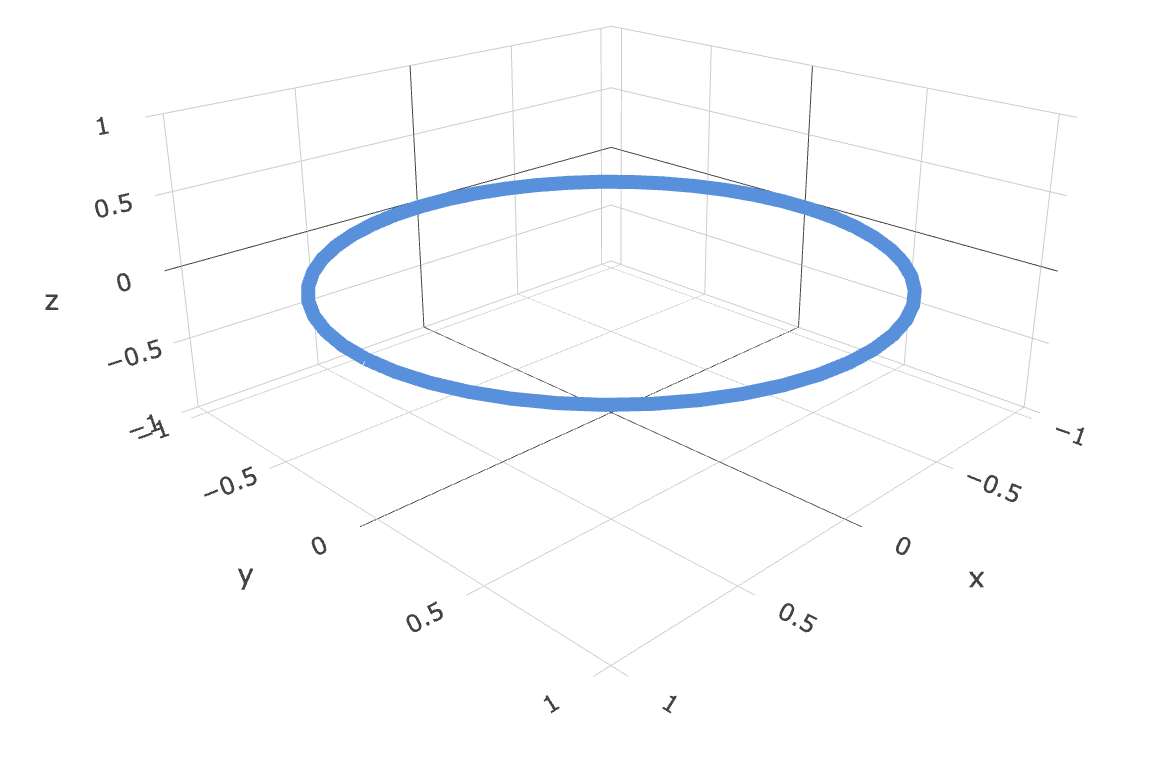
\includegraphics[width=0.3\linewidth]{figures/space-curve-circ.png}
    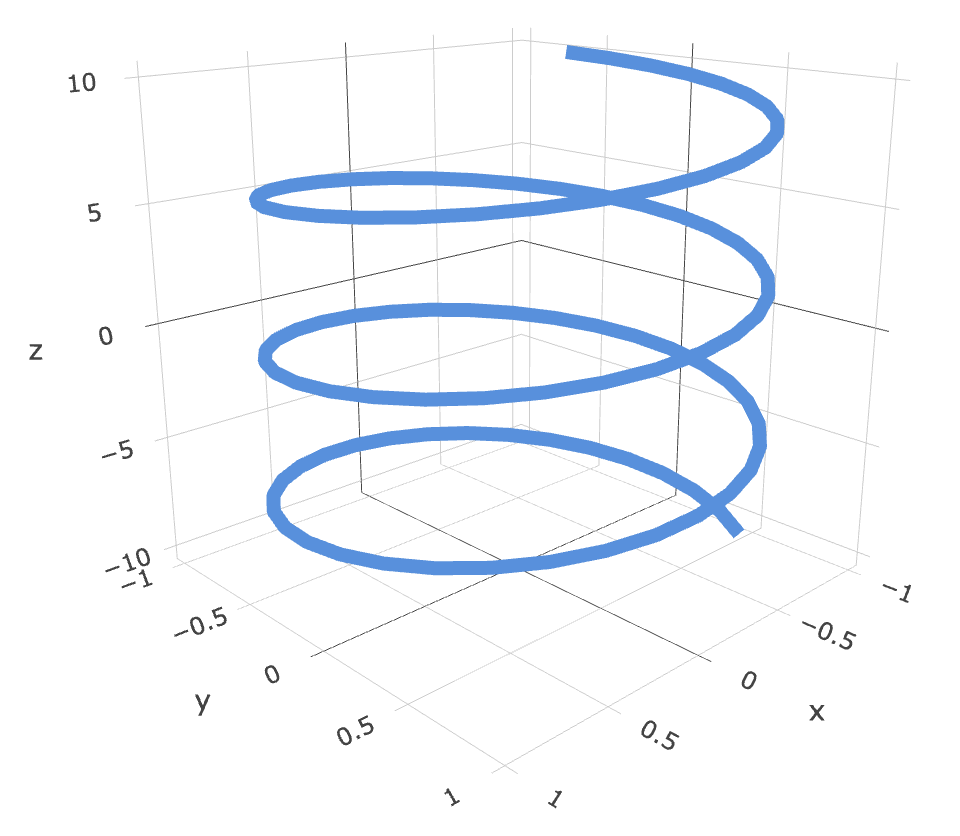
\includegraphics[width=0.3\linewidth]{figures/space-curve-helix.png}
    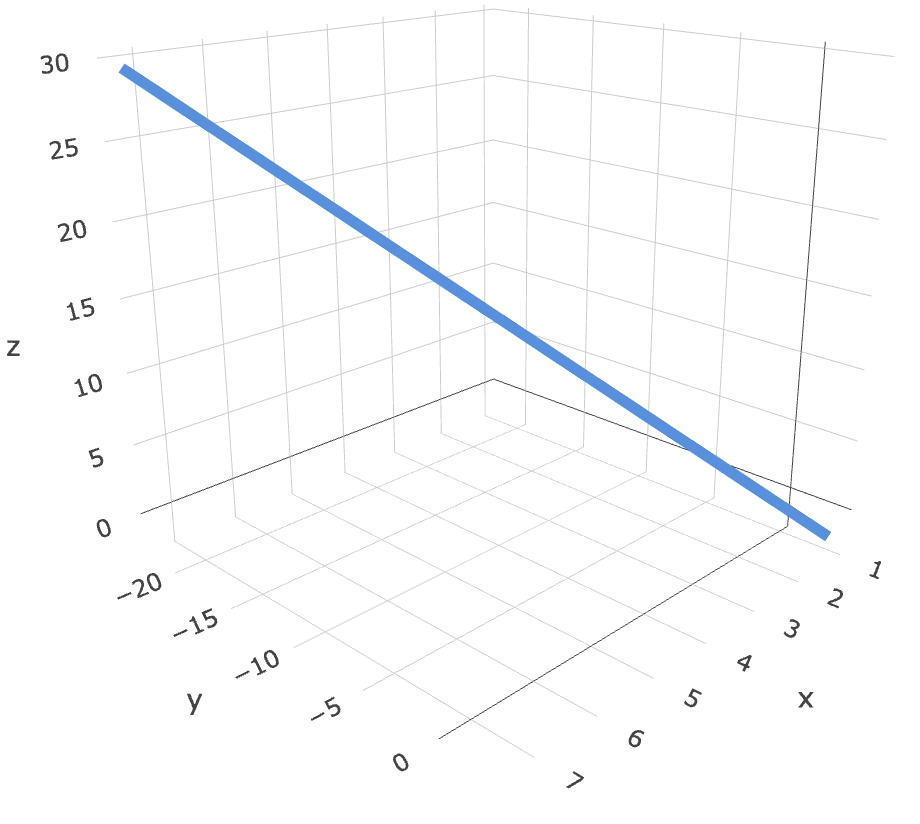
\includegraphics[width=0.3\linewidth]{figures/space-curve-line.png}
    \caption{Examples of space curves}
    \label{fig:space_curves}
\end{figure}
\end{example}

\section{Derivatives and Integrals of Vector Functions}

\subsection{Derivatives}

\begin{definition}[Derivative of vector functions]
$$
\frac{d\mathbf r}{dt} = \mathbf{r}'(t) = \lim_{h\to0}\frac{\mathbf{r}(t+h)-\mathbf{r}(t)}{h}
$$
\end{definition}

If follows from the definition of vector function that
$$
r'(t)= (f'(t),\, g'(t),\, h'(t))
$$

In 2D, the derivative at a point gives us the slope of the tangent line to the graph at that point. Similarly, the derivative of a vector function at a given point gives us a vector that is tangent to the curve.

\begin{figure}[h]
    \centering
    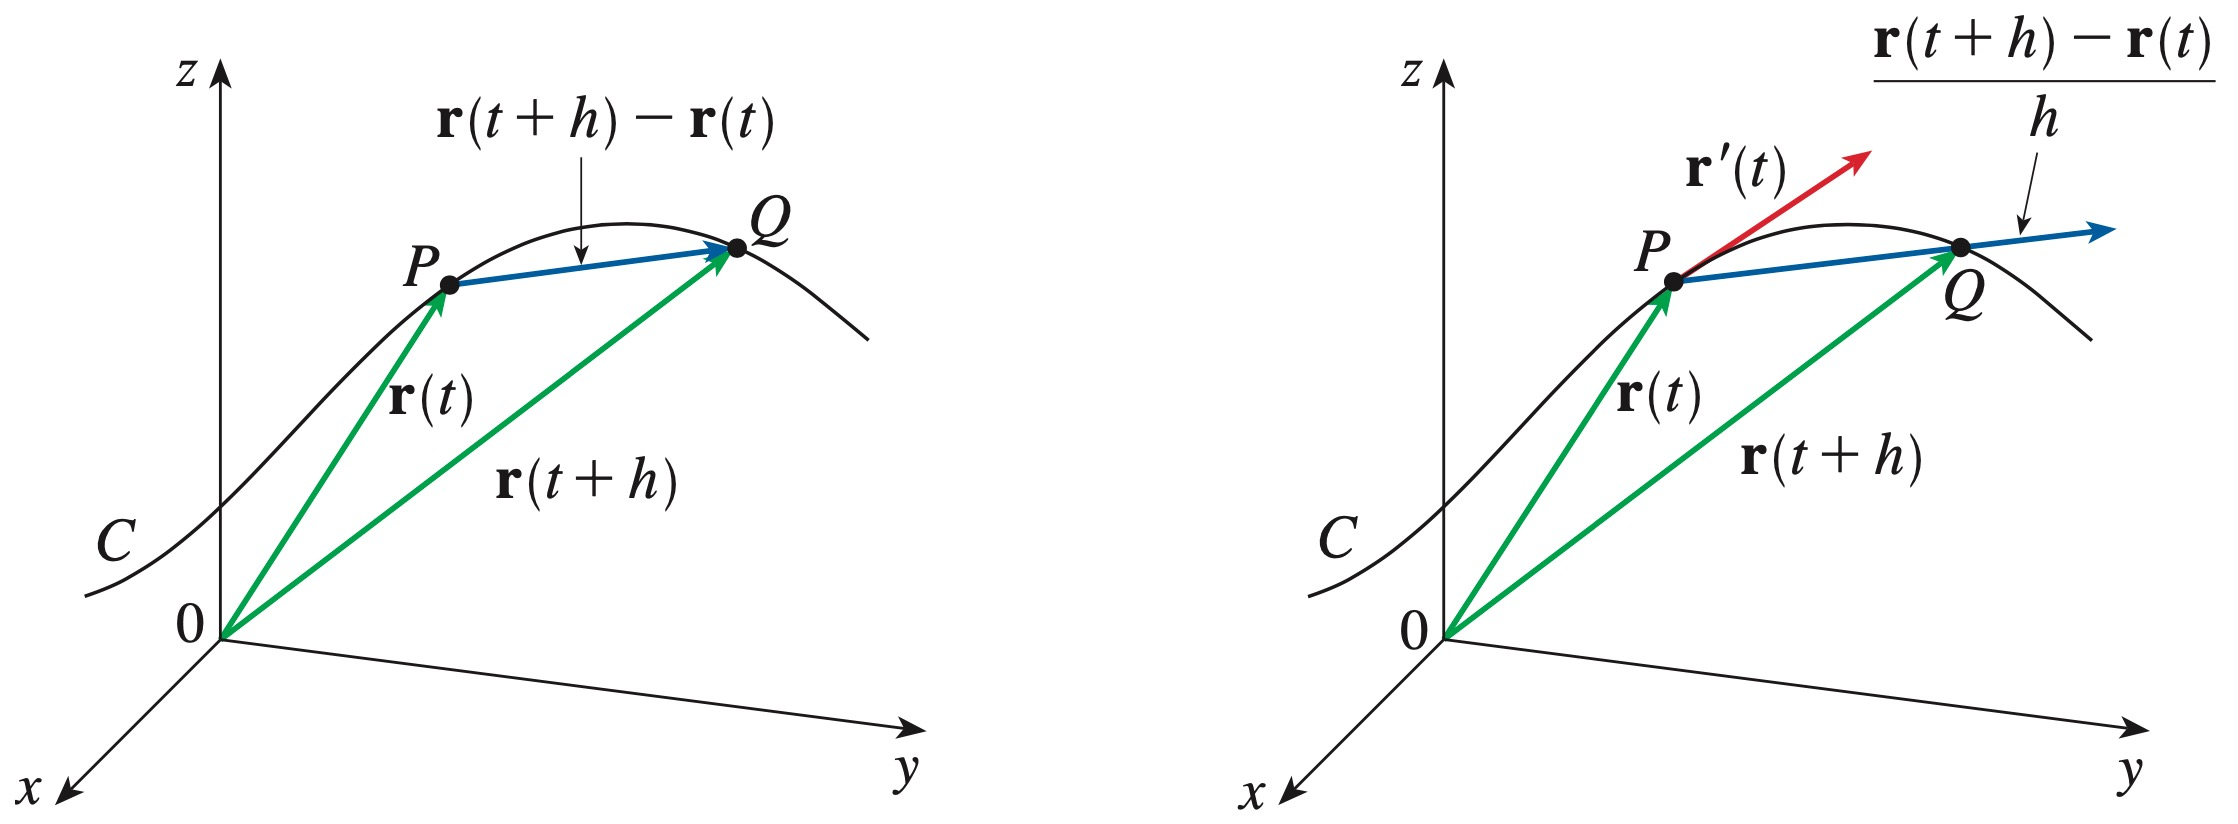
\includegraphics[width=0.6\linewidth]{figures/tangent-vector.jpeg}
    \caption{Secant and tangent vector}
    \label{fig:tan_vec}
\end{figure}

A unit vector that has the same direction as the vector tangent to the curve is called the {\bf unit tangent vector} or simply {\bf tangent vector}, denoted $T$.
$$
T(t) = \frac{r'(t)}{\norm{r'(t)}}
$$

The differentiation rules are mostly the same as real-value functions. There are some variants of the product rule, as shown below:
\begin{theorem}
\begin{multicols}{2}
    \begin{enumerate}
        \item $\displaystyle\frac{d}{dt}\left[ f(t) \mathbf{u}(t) \right] = f'(t)\mathbf{u}(t) + f(t)\mathbf{u}'(t)$
        \item $\displaystyle\frac{d}{dt}\left[ \mathbf{u}(t) \cdot \mathbf{v}(t) \right] = \mathbf{u}'(t)\cdot\mathbf{v}(t) + \mathbf{u}(t)\cdot\mathbf{v}'(t)$
        \item $\displaystyle\frac{d}{dt}\left[ \mathbf{u}(t) \times \mathbf{v}(t) \right] = \mathbf{u}'(t)\times\mathbf{v}(t) + \mathbf{u}(t)\times\mathbf{v}'(t)$
    \end{enumerate}
\end{multicols}
\end{theorem}

\begin{lemma} \label{lem:derivative_sphere}
Let $r(t)$ be a vector function such that $\norm{r(t)}=c$ where $c$ is a constant for all $t$ in the domain. Then, $r(t)$ is orthogonal to $r'(t)$. In other words,
$$
r(t) \cdot r'(t) = 0
$$
\begin{figure}[h]
    \centering
    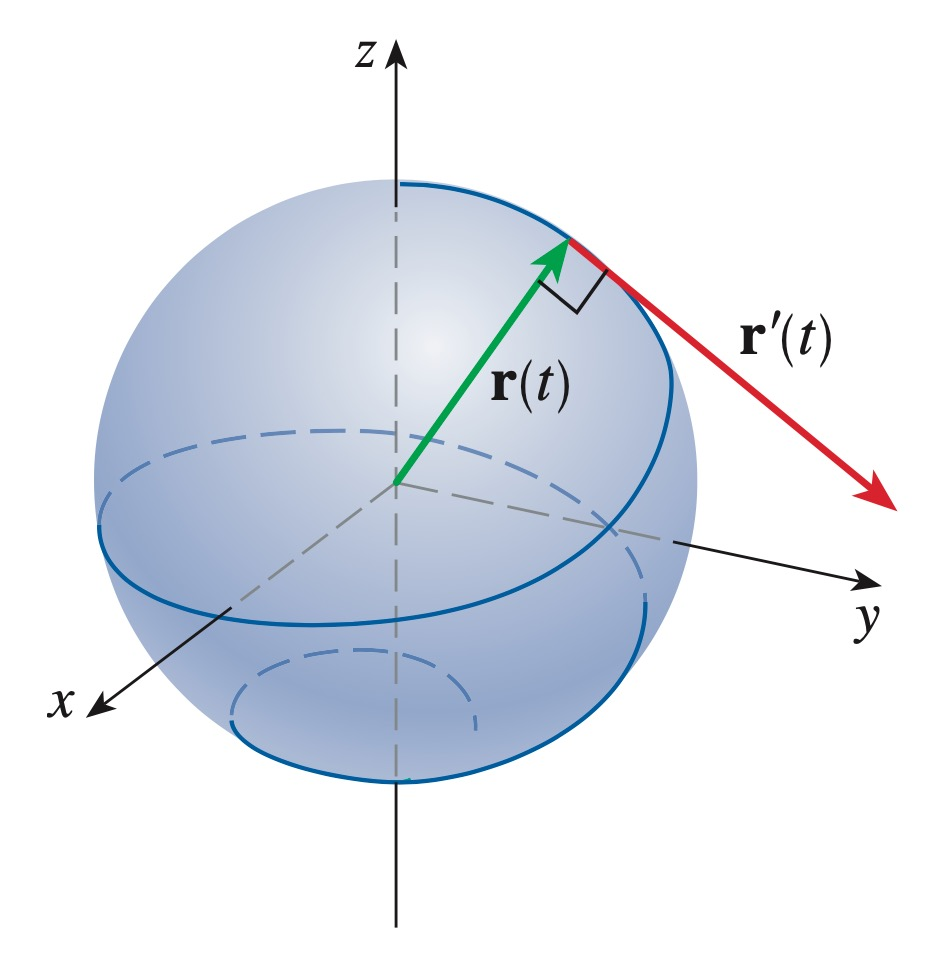
\includegraphics[width=0.3\linewidth]{figures/sphere.jpeg}
    \caption{$r(t)$ will be a function on the surface of a sphere of radius $c$}
    \label{fig:derivative_sphere}
\end{figure}
\end{lemma}

Proof of Lemma \ref{lem:derivative_sphere}

\begin{proof}
\hfill \\
Since $\norm{r(t)} = c$, we can square both sides to get
$$
\norm{r(t)}^2 = c^2
$$
from which we can introduce the dot product
\begin{align*}
    r(t) \cdot r(t) = c^2
\end{align*}
Differentiate both sides
\begin{align*}
    \frac{d}{dt} [r(t) \cdot r(t)] &= \frac{d}{dt} c^2 \\
    r(t) \cdot r'(t) + r'(t) \cdot r(t) &= 0 \\
    2r(t)\cdot r'(t) &= 0 \\
    r(t) \cdot r'(t) &= 0
\end{align*}
\end{proof}

\subsection{Integral}

\begin{definition}[Integral of vector functions]
$$
\int_a^b \mathbf{r}(t)dt = \lim_{n\to\infty}\sum_{i=1}^n \mathbf{r}(t_i^*)\Delta t
$$
\end{definition}
Again, it follows from the definition of vector function that
$$
\int_a^b \mathbf{r}(t)dt = \left(\int_a^b f(t)dt,\; \int_a^b g(t)dt,\; \int_a^b h(t)dt \right)
$$
The integral of a vector function is also a vector. It does not have an obvious geometric meaning.

In physics, we can integrate the acceleration vector to get the velocity vector, and integrate the velocity vector to get the displacement vector.

\section{Arc Length}

Consider each tiny line segment on the curve. Using the Pythagorean's theorem, we know that the length of each segment is
\begin{align*}
    \sqrt{(x_{i+1}-x_i)^2 + (f(x_{i+1}-f(x_i))^2}
\end{align*}
Multiply by $\frac{(x_{i+1}-x_i)}{(x_{i+1}-x_i)}$
\begin{align*}
    (x_{i+1}-x_i) \sqrt{\frac{(x_{i+1}-x_i)^2}{(x_{i+1}-x_i)^2} + \frac{(f(x_{i+1}-f(x_i))^2}{(x_{i+1}-x_i)^2}} \\
\end{align*}
Then, the arc length is just the infinite sum of all infinitely small line segments,
\begin{align*}
    L &=\lim_{n\to\infty} \left[\sum_{i=1}^n (x_{i+1}-x_i) \sqrt{\frac{(x_{i+1}-x_i)^2}{(x_{i+1}-x_i)^2} + \frac{(f(x_{i+1}-f(x_i))^2}{(x_{i+1}-x_i)^2}} \right] \\
    &= \int_a^b \sqrt{1+[f'(x)]^2} dx
\end{align*}
Hence, for 2D parametric curves,
$$
L = \int_a^b \sqrt{\left( \frac{dx}{dt} \right)^2 + \left( \frac{dy}{dt} \right)^2} dt
$$
Similarly, for 3D,
$$
L = \int_a^b \sqrt{\left( \frac{dx}{dt} \right)^2 + \left( \frac{dy}{dt} \right)^2 + \left( \frac{dz}{dt} \right)^2} dt
$$

\begin{theorem}[Arc length]
The arc length between $a$ and $b$ for a vector function (parametric curve) in 3D is
$$
L = \int_a^b \sqrt{\left( \frac{dx}{dt} \right)^2 + \left( \frac{dy}{dt} \right)^2 + \left( \frac{dz}{dt} \right)^2} dt = \int_a^b \norm{\mathbf{r}'(t)}dt
$$
\end{theorem}

\begin{example}
Find the arc length of $r(t) = (\cos\frac{t}{\sqrt 2}, \sin\frac{t}{\sqrt 2}, \frac{t}{\sqrt 2})$ for $0 \leq t \leq 1$.
$$
L = \int_0^2 \norm{r'(t)}dt = \int_0^2 1 dt = 2
$$
\end{example}

\section{Reparameterization w.r.t. Arc Length}

We can change the parameter by transform the domain. Suppose we have $r(t) = (t,2t^2,3t^3)$ for $1 \leq t \leq 5$.

If we define $s = e^t$, then $r(s) = (e,2e^2,3e^3)$ for $0 \leq s \leq \ln 5$. Note that this only works with continuous functions (in this case $e^t$).

Let $s$ be a function that takes $t$ as an input, and outputs the arc length between some point $a$ and $t$. Since 
$$
s(t) = \int_a^t \norm{r'(u)} du
$$
by the Fundamental Theorem of Calculus,
$$
\frac{ds}{dt} = \frac{d}{dt}\int_a^t \norm{r'(u)}du = \norm{r'(t)}
$$

Let $s^{-1}$ be the inverse of $s$ on the relevant interval. Then,
$$
s^{-1}(s(t)) = t \quad \text{ and } \quad s(s^{-1}(s))=s
$$
Differentiate both sides and apply the Chain Rule
$$
\frac{ds}{dt} = \frac{1}{(s^{-1})'(s(t))} \qquad \frac{ds^{-1}}{ds}=\frac{1}{s'(s^{-1}(s))}
$$
Let $q(s)=r(s^{-1}(s))$. $q(s)$ is called the arc length parameterization of $r(t)$.

The arc length parameterization has some really neat properties. Because $ds = \norm{r'(t)}dt$,
$$
L = \int \norm{r'(t)} dt = \int_a^b ds = b-a
$$

To show that $q$ is an arc length parameterization, we just need to show that
$$
\norm{q'(s)} = \left\lVert{\frac{d}{dt} r(s^{-1}(s))}\right\rVert = \norm{(s^{-1})'(s) \cdot r'(s^{-1}(s))} = \left\lVert \frac{r'(s^{-1}(s))}{s'(s^{-1}(s))} \right\rVert = \left\lVert \frac{r'(t)}{r'(t)} \right\rVert = 1
$$

For a vector function parameterized by arc length, the tip of the vector travels at a constant rate of one unit of arc length per unit of time. This is similar to the notion of radian, which is defined as $1 \mathrm{rad} = 1 \text{ unit of arc length}$ in a unit circle.

Despite the nice properties, it is often hard or even impossible to analytically find the arc length parameterization.

\begin{example}[Arc length parameterization]
\begin{enumerate}
    \item Unit circle: $r(t) = (\cos t, \sin t, 0)$. In this case, $r$ is already parameterized with respect to arc length. So, $s=t$, and $r(s) = (\cos s, \sin s, 0)$. This is the definition of radian measure.
    \item Helix: $r(t) = (\cos t, \sin t, t)$. Calculate the arc length:
    $$
    s = \int_0^t \norm{r'(u)}du = \int_0^t \sqrt{\cos^2 u + \sin^2 u + 1} du = \sqrt{2}t
    $$
    Solve for the inverse of $s$, which gives $t= s/\sqrt2$. Hence the arc length parameterization:
    $$
    r(s) = \left( \cos\frac{s}{\sqrt2},\; \sin\frac{s}{\sqrt2},\; \frac{s}{\sqrt2} \right)
    $$
\end{enumerate}
\end{example}

\section{Curvature}

\begin{definition}[Smoothness]
Given a function $r(t)$, a parameterization is called smooth on an interval $I$ if $r'(t) \neq 0$. A curve is called smooth if it has a smooth parameter. A smooth curve has no sharp corners or cusps.
\end{definition}

\begin{definition}[Curvature]
The curvature of a curve is
$$
\kappa = \left\lVert{\frac{dT}{ds}}\right\rVert
$$
\end{definition}

Notice that $\kappa$ depends on the arc length parameterization. We can calculate this number as
$$
\frac{dT}{ds} = \frac{dT}{ds} \cdot 1 = \frac{dT}{ds}\cdot \frac{dt}{dt} = \frac{dT}{dt} \cdot \frac{dt}{ds}
$$
Since $ds/dt = \norm{r'(t)}$,
$$
\frac{dT}{ds} = \frac{dT/dt}{ds/dt} = \frac{dT/dt}{\norm{r'(t)}}
$$
Hence,
$$
\kappa = \frac{\norm{dT/dt}}{\norm{r'(t)}}
$$
which is now independent of the arc length parameterization $s$.

\begin{example}
The curvature of a circle of length $a$.

The equation of that circle is $r(t) = (a\cos t, a\sin t)$. Therefore, $r'(t)=(-a\sin t,a \cos t)$ and $\norm{r'(t)}=a$.

So,
$$
T(t)=\frac{r'(t)}{\norm{r'(t)}} = (-\sin t, \cos t)
$$
and
$$
T'(t)=(-\cos t, -\sin t)
$$
This gives $\norm{T'(t)} = 1$ and hence
$$
\kappa = \frac{T'(t)}{r'(t)} = 1/a
$$
This result also implies that circle has constant curvature, and that smaller circle has larger curvature.
\end{example}

\begin{theorem} \label{eq:alt_curvature}
The curvature can also be calculated as follows:
$$
\kappa(t) = \frac{\norm{r'(t) \times r''(t)}}{\norm{r'(t)}^2}
$$
and for plane curves of the form $y = f(x)$, we can choose $x$ as the parameter and write $r(x) = (x,f(x))$. Then,
$$
r'(x) = (1, f'(x)) \qquad r''(x)=(0,f''(x))
$$
And $\norm{r'(x)} = \sqrt{1+[f'(x)]^2}$. Hence, by the previous equation \eqref{eq:alt_curvature}
$$
\kappa(x) = \frac{\norm{f''(x)}}{\left[ 1+(f'(x))^2 \right]^{3/2}}
$$
\end{theorem}

\section{Normal and Binormal Vectors}

\begin{definition}[Normal vector]
Given a function $r(t)$, we know that $T(t) = \frac{r'(t)}{\norm{r'(t)}}$ is a unit vector called the tangent vector. Recall that by Lemma \ref{lem:derivative_sphere} if $\norm{r(t)}=c$ where $c$ is a constant, then $r(t)\cdot r'(t) = 0$.

Since $\norm{T(t)}=1$, we can conclude that $T(t)$ is perpendicular to $T'(t)$. We define the (unit) normal vector as
$$
N(t) = \frac{T'(t)}{\norm{T'(t)}}
$$
which is normal to $T(t)$.
\end{definition}

\begin{definition}[Binormal vector]
We define the binormal vector $B$ as the cross product between $T$ and $N$.
$$
B(t) = T(t) \times N(t)
$$
which is also a unit vector so $\norm{B(t)}=1$.
\end{definition}

\begin{figure}[h]
    \centering
    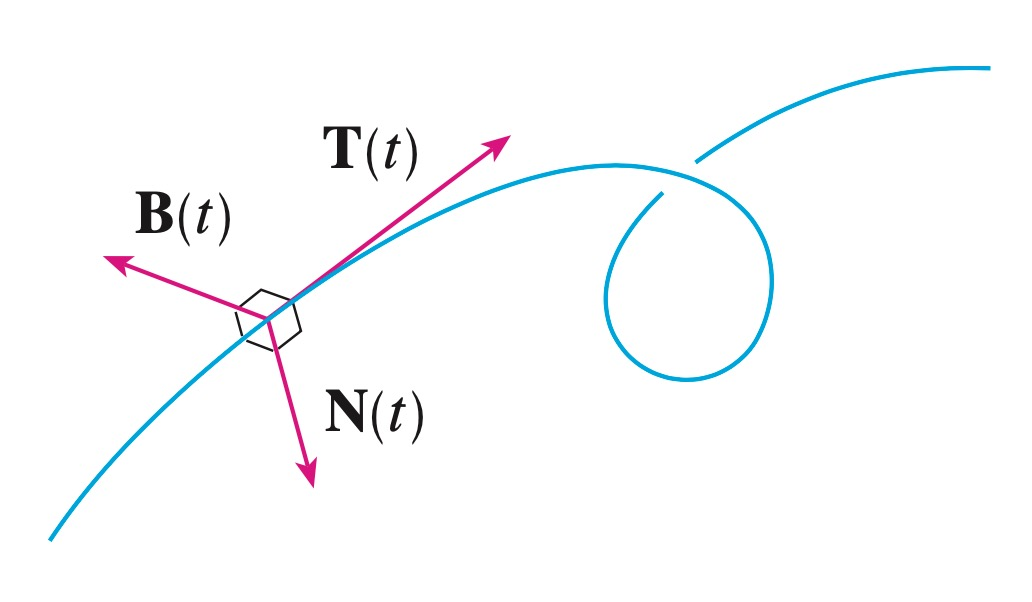
\includegraphics[width=0.3\linewidth]{figures/normal-binormal.jpeg}
    \caption{Normal and Bionormal function}
    \label{fig:normal_binormal_vec}
\end{figure}

$T,N,B$ together define a new set of axes. $B$ defines the binormal line, and $N$ defines the normal line.

In addition, the plane between $N$ and $T$ is called the osculating plane. The plane between $B$ and $T$ is called the rectifying plane. The plane between $N$ and $B$ is called the normal plane.

\begin{figure}[h]
    \centering
    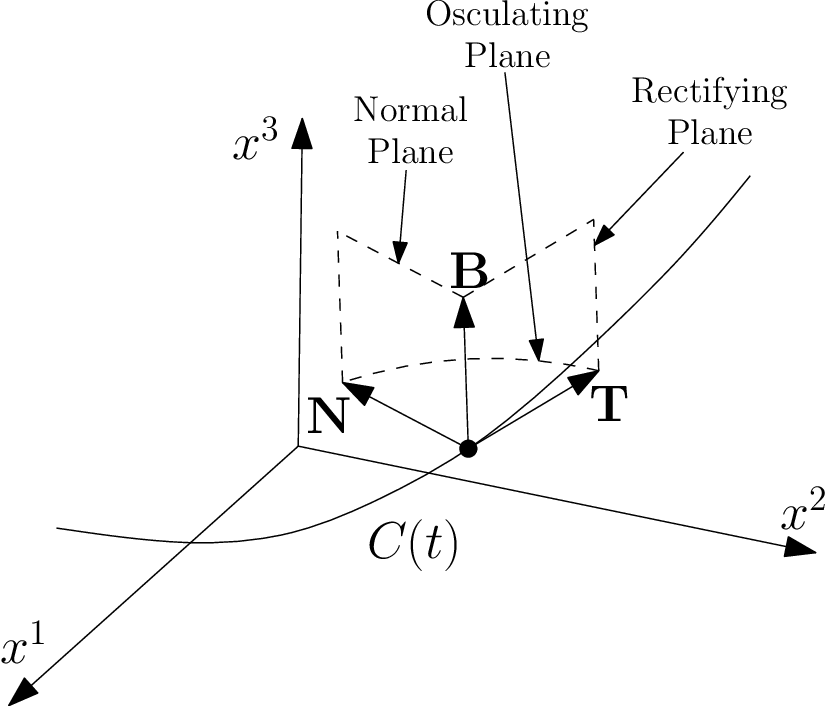
\includegraphics[width=0.4\linewidth]{figures/NTB-planes.png}
    \caption{Normal, osculating, and rectifying planes}
    \label{fig:NTB_planes}
\end{figure}

\section{Torsion}